\selectlanguage{ngerman}%
\frenchspacing%
\begin{ledgroupsized}[r]{120mm}
\footnotesize
\pstart
\noindent\textbf{Überlieferung:}
\pend
\end{ledgroupsized}
\begin{ledgroupsized}[r]{114mm}
\footnotesize
\pstart \parindent -6mm
\makebox[6mm][l]{\textit{L}}%
\edlabel{LH_37_05_043_ueberliefer-1}%
Aufzeichnung:
LH XXXVII~5 Bl.\;43.
Ein Blatt 8\textsuperscript{o},
Ränder beschnitten;
Papiererhaltungsmaßnahmen.
Gleiches Papier wie N.\;\ref{60142+60297},
Zeuge \textit{L\textsuperscript{2}}.
Zwei Seiten.
Der Anfang von N.\;\ref{60299} (unten, \refpassage{LH_37_05_043r_anfang-1}{LH_37_05_043r_anfang-2}: \textit{Directio conatuum ... quam ut}) überliefert mit wenigen Abweichungen den gleichen Text wie der Anfang von N.\;\ref{60142+60297}, Zeuge \textit{L\textsuperscript{1}} (vgl. \refpassage{60142+60297_anfang-1}{60142+60297_anfang-2} samt Varianten).%
\edlabel{LH_37_05_043_ueberliefer-2}
\pend
\end{ledgroupsized}
\vspace{5mm}%
\normalsize%
\pstart%
\noindent%
\lbrack%
\edtext{%
\href{\Scan{LH_37_05_043r}}%
{43\,r\textsuperscript{o}}%
\rbrack\ %
\edlabel{LH_37_05_043r_anfang-1}
Directio%
}{%
\lemma{\lbrack\href{\Scan{LH_37_05_043r}}{43\:r\textsuperscript{o}}\rbrack}%
\Bfootnote{%
\textit{(1)}~Praeter
\textit{(2)}~Directio%
~\textit{L}}}
conatuum%
\indexS{directio conatus duplex}%
\indexS{conatus eccentricus}
\edtext{corporis}{%
\lemma{}\Bfootnote{%
corporis
\textit{erg.\:L}}}
duplex est,
centralis%
\indexS{directio conatus centralis}
et Eccentrica.%
\indexS{directio conatus eccentrica}
Centralis est
cum linea directionis%
\indexS{linea directionis}
incidit in centrum gravitatis%
\indexS{centrum gravitatis corporis impulsi}
\edtext{ipsius corporis}{%
\lemma{}\Bfootnote{%
ipsius corporis
\textit{erg.\:L}}}
seu cum recta perpendicularis%
\indexS{recta perpendicularis ad contactum}%
\indexS{contactus corporis impellentis et impulsi}
\edtext{ad contactum}{%
\lemma{ad}\Bfootnote{%
\textit{(1)}~tangentem
\textit{(2)}~contactum%
~\textit{L}}}
impellentis et impulsi%
\indexS{corpus impellens}%
\indexS{corpus impulsum}
producta transit per centrum gravitatis impulsi;%
\indexS{centrum gravitatis corporis impulsi}
tunc enim directio%
\indexS{directio corporis impulsi}
\edtext{%
quam corpus impulsum accipit,%
}{%
\lemma{quam}\Bfootnote{%
\bars{corpus \textit{erg.}}
impulsum
\textit{(1)}~accidit,
\textit{(2)}~accipit,%
~\textit{L}}}
dicetur centralis;%
\indexS{directio conatus centralis}
sin minus, Eccentrica.%
\indexS{directio conatus eccentrica}
\pend%
\vspace{1.40em}%
\centerline{\hspace{-45mm}%
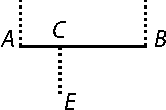
\includegraphics[width=0.19\textwidth]{gesamttex/edit_VIII-4/images/LH_37_05_043_d1_043r.pdf}}%
\vspace{0.25em}%
\centerline{\hspace{-45mm}%
\lbrack\textit{Fig.\:1}\rbrack}
\vspace{-5.82em}%
\centerline{\hspace{45mm}%
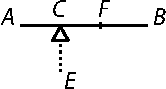
\includegraphics[width=0.19\textwidth]{gesamttex/edit_VIII-4/images/LH_37_05_043_d2_043r.pdf}}%
\vspace{0.25em}%
\centerline{\hspace{45mm}%
\lbrack\textit{Fig.\:2}\rbrack}
\vspace{1.0em}
\pstart%
Cum centralis est directio,%
\indexS{directio conatus centralis}
satis
\edtext{explicuimus}{%
\lemma{explicuimus}\Cfootnote{%
Siehe die Erläuterung zu N.\;\ref{60142+60297}, \refpassage{LH_35_10_17_009+37_05_041_explicuimus-1}{LH_35_10_17_009+37_05_041_explicuimus-2}.%
}}
ejus eventa,
perinde enim est,
ac si con\-ci\-pe\-re\-mus mobile
velut collectum in punctum,%
\indexS{mobile collectum in punctum}
nempe in centrum gravitatis.%
\indexS{mobile collectum in centrum gravitatis}
Sed Ec\-cen\-tri\-ca altioris est indaginis;%
\indexS{directio conatus eccentrica}%
\indexS{indago altior}%
\indexS{indago de directione conatus eccentrica}
quam ut%
\edlabel{LH_37_05_043r_anfang-2}
melius intelligamus,
utemur exemplo faciliore,%
\indexS{exemplum facilius}
lineae scilicet rectae \textit{ACB}
quae impellatur directione \textit{EC}.%
\indexS{linea recta impulsa}
Quaeritur quid sit futurum.
Eadem autem res redit,
ac si poneremus lineam \textit{AB}
incurrere in obstaculum \textit{C}.%
\indexS{obstaculum}%
\indexS{linea incurrens in obstaculum}
Quo facto
\edtext{conatus partium%
\indexS{conatus partium}%
}{%
\lemma{}\Bfootnote{%
conatus
\bars{ipsarum \textit{gestr.}}
partium%
~\textit{L}}}
\textit{CA} et \textit{CF} se
\edtext{mutuo compensabunt,%
\indexS{conatus compensantes se mutuo}
et conjungentur%
\indexS{conjunctio directionis centralis et circulationis}%
}{%
\lemma{mutuo}\Bfootnote{%
\textit{(1)}~destruent; et con
\textit{(2)}~compensabunt, et
\textit{(a)}~concur
\textit{(b)}~conjungentur%
~\textit{L}}}
directio centralis ipsius \textit{AF},%
\indexS{directio conatus centralis}
cujus centrum \textit{C},
et praeterea circulatio ipsius \textit{FB} circa \textit{C}.
Sed ubi paulum inclinata est \textit{AB}
per circulationem%
\indexS{circulatio in concursu eccentrico}
\edtext{circa \textit{C},%
}{%
\lemma{}\Bfootnote{%
circa \textit{C}
\textit{erg.\:L}}}
ita ut angulus \textit{ACE} fiat obtusus,%
\indexS{angulus obtusus}
jam simul et circulatur \textit{AB} circa \textit{C},
et progreditur glissando
\edtext{%
super \textit{C}.
\ledpb%
Fit etiam repercussio%
\indexS{repercussio ob obstaculum}%
\indexS{repercussio ob vim respectivam}
ab obstaculo,%
\indexS{obstaculum}
ob vim respectivam;%
\indexS{vis respectiva}
sed nobis sufficit%
\lbrack,\rbrack\
sine omni ictu,%
\indexS{ictus}
simplices%
}{%
\lemma{super \textit{C}.}\Bfootnote{%
\textit{(1)}~Sed nobis
\textit{(2)}~Fit etiam
\lbrack...\rbrack\ nobis sufficit
\textit{(a)}~si
\textit{(b)}~sine omni ictu, simplices%
~\textit{L}}}
nisus%
\indexS{nisus simplex}%
\indexS{nisus sine ictu}
\edlabel{LH_37_05_043_m043r1}%
considerare.
\edtext{}{%
\xxref{LH_37_05_043_m043r1}{LH_37_05_043_m043r2}%
\lemma{considerare.}\Bfootnote{%
\textit{(1)}~Idque
\textit{(2)}~Si \textit{AB}%
~\textit{L}}}%
\lbrack%
\href{\Scan{LH_37_05_043v}}%
{43\,v\textsuperscript{o}}%
\rbrack%
\pend%
\pstart%
Si%
\edlabel{LH_37_05_043_m043r2}
\edtext{\textit{AB} sustineatur}{\lemma{\textit{AB} sustineatur}\Cfootnote{%
Vgl. das Diagramm \lbrack\textit{Fig.\:3}\rbrack.}}
in \textit{C},
sumatur $CF=AC$,
et supererit nisus%
\indexS{nisus superstes}
ipsius \textit{FB} secundum nisum centri%
\indexS{nisus centri gravitatis}%
\indexS{centrum gravitatis corporis sustenti}
sui gravitatis \textit{H},
quo conabitur \textit{H} moveri circa \textit{C}
ita
\edtext{ut celeritas conatus circulatorii%
\indexS{conatus circulatorius}%
\indexS{celeritas conatus circulatorii}%
}{%
\lemma{ut}\Bfootnote{%
\textit{(1)}~conatus circ
\textit{(2)}~celeritas
\textit{(a)}~circulationis
\textit{(b)}~conatus circulatorii%
~\textit{L}}}
puncti \textit{H} sit aequalis celeritati
qua inciperet descendere \textit{H}
si non retineretur,
seu celeritati ipsius%
\indexS{impressio}%
\indexS{celeritas impressionis}
\edlabel{LH_37_05_043_m043v1}%
impressionis.%
\edtext{}{%
\xxref{LH_37_05_043_m043v1}{LH_37_05_043_m043v2}%
\lemma{impressionis.}\Bfootnote{%
\lbrack/\rbrack\
\textit{(1)}~Sed \textlangle\textit{C}\textrangle\ qui
\lbrack/\rbrack\
\textit{(2)}~Motus perinde
\textit{(a)}~erit
\textit{(b)}~aequalem exhibemus
\textit{(3)}~\bars{Se \textit{streicht Hrsg.}}
\textit{(4)}~\textit{C} premitur %
\lbrack...\rbrack\ \textit{AF}, sed%
~\textit{L}}}
\textit{C} premitur pondere%
\indexS{pondus premens}
ipsius \textit{AF},
sed%
\edlabel{LH_37_05_043_m043v2}
non pondere ipsius \textit{FB},
quod libere agit.%
\indexS{pondus agens libere}
\edlabel{LH_37_05_043_043v_centrgyr-1}%
Eodem igitur modo res se habet
cum impulsu \textit{C},%
\indexS{impulsus eccentricus}
ut eo solum afficiatur
\edlabel{LH_37_05_043_043v_cdrb-1}%
\edtext{}{%
\lemma{\textit{AF}}\Bfootnote{%
\textit{(1)}~. Sed si ponamus descendere \textit{H}
\textit{(2)}~reliquo \textit{FB} %
\lbrack...\rbrack\ puncto \textit{H},
\textit{(a)}~moveatur \textit{C} ea celeritate quam nisus pu
\textit{(b)}~punctum \textit{C} habet conatum impulsus.
\textit{(aa)}~\lbrack/\rbrack\ Hinc si
\textit{(bb)}~Adeoque gyratur %
\lbrack...\rbrack\ Idem est%
~\textit{L}}}%
\textit{AF}
reliquo \textit{FB} non affecto,
ac proinde quiescente puncto \textit{H},
punctum \textit{C} habet conatum impulsus.%
\indexS{conatus impulsus}
Adeoque gyratur \textit{C}
circa \textit{H}
celeritate impulsus.%
\indexS{celeritas impulsus}%
\indexS{impulsus eccentricus}%
\edlabel{LH_37_05_043_043v_centrgyr-2}
\pend%
\vspace{2.5em} %
\centerline{%
\hspace{-55mm}%
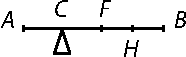
\includegraphics[width=0.20\textwidth]{gesamttex/edit_VIII-4/images/LH_37_05_043_d3_043v.pdf}}
\vspace{1.00em}
\centerline{%
\hspace{-55mm}%
\lbrack\textit{Fig.\:3}\rbrack}
\vspace{1em}
\vspace{-7.45em} %
\centerline{%
\hspace{55mm}%
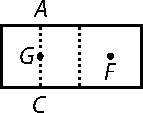
\includegraphics[width=0.15\textwidth]{gesamttex/edit_VIII-4/images/LH_37_05_043_d4_043v.pdf}}
\vspace{0.25em}
\centerline{%
\hspace{55mm}%
\lbrack\textit{Fig.\:4}\rbrack}
\vspace{1.15em}%
\pstart%
\edlabel{LH_37_05_043_043v_urzelle-1}%
Idem est%
\edlabel{LH_37_05_043_043v_cdrb-2}
in toto aliquo corpore,
ut si
\edtext{corpus %
impellitur%
\indexS{corpus impulsum}%
}{%
\lemma{corpus %
impellitur}\Cfootnote{%
Vgl. das Diagramm \lbrack\textit{Fig\:4}\rbrack.}}
impulsu \textit{C},%
\indexS{impulsus eccentricus}
habebitur \textit{G} centrum impulsi%
\indexS{centrum gravitatis corporis impulsi}%
\indexS{corpus impulsum}
et gyrantis%
\indexS{centrum gravitatis corporis gyrantis}%
\indexS{corpus gyrans}
ac \textit{F} centrum reliqui%
\indexS{corpus reliquum}%
\indexS{centrum gravitatis corporis reliqui}
circa quod fit gyratio.%
\indexS{gyratio circa centrum corporis reliqui}%
\edlabel{LH_37_05_043_043v_urzelle-2}
Puncti concursus%
\indexS{punctum concursus}%
\indexS{concursus corporum}
planorum,%
\indexS{planum concursus}
hic nulla habenda ratio.
\pend%
\pstart%
Dubia interdum fit perpendicularis ad contactum%
\indexS{contactus corporum concurrentium}%
\indexS{linea perpendicularis ad contactum}%
\lbrack,\rbrack\
ut si
\edtext{\textit{a} et \textit{b} corpora}{%
\lemma{\textit{a}~et~\textit{b} corpora}\Cfootnote{%
Vgl. das Diagramm \lbrack\textit{Fig.\:5}\rbrack.}}
concurrant;
multae enim duci
\edtext{%
possunt tangentes utrumque corpus
in puncto communi,%
\indexS{punctum commune}%
\indexS{linea tangens in puncto communi}
ut \textit{lm}, \textit{no},%
}{%
\lemma{possunt}\Bfootnote{%
\textit{(1)}~perpendiculares ad contactum, ut \textit{l}
\textit{(2)}~tangentes utrumque %
\lbrack...\rbrack\ ut \textit{lm}, \textit{no},%
~\textit{L}}}
nec proinde haec plane finita.
\pend%
\pstart%
Sit%
\indexS{pondus sustentatum}
\edtext{pondus \textit{A}}{%
\lemma{pondus \textit{A}}\Cfootnote{%
Vgl. das Diagramm \lbrack\textit{Fig.\:6}\rbrack.}}
sustentatum fulcris%
\indexS{fulcrum innitens}
\edtext{%
\textit{LM}, \textit{PQ}
quae innituntur brachiis \textit{NM},%
\indexS{brachium sustinens}
\lbrack\textit{RQ}\rbrack\
et sustinentur ponderibus \textit{B}, \textit{C} %
ex brachiis \textit{BN}, \textit{CR}.%
\indexS{pondus sustinens}%
\indexS{brachium sustinens}
Ponantur autem \textit{BN}, \textit{CR}, \textit{RQ}, \textit{NM} aequales.
Quaeritur quae debeat esse ratio%
}{%
\lemma{\textit{LM}, \textit{PQ}}\Bfootnote{%
\textit{(1)}~quaeritur quomodo se habere debeat
\textit{(2)}~quae innituntur brachiis \textit{NM},
\bars{\textit{RC} \textit{ändert Hrsg.}}
et sustinentur %
\lbrack...\rbrack\ Ponantur autem
\textit{(a)}~\textit{BN}, \textit{NM},
\textit{(b)}~\textit{BC} f
\textit{(c)}~\textit{BN}, \textit{CR}, %
\lbrack...\rbrack\ esse ratio%
~\textit{L}}}
cujusque ponderis \textit{B} et \textit{C} ad pondus \textit{A}.
\pend%
\newpage%
\pstart%
Comparetur haec consideratio
cum consideratione motus compositi%
\indexS{motus compositus e volutione et defluxu}
ex volutione%
\indexS{volutio globi}
et defluxu globi%
\indexS{defluxus globi}
super plano inclinato.%
\indexS{planum inclinatum}
Nam et in impulsu eccentrico%
\indexS{impulsus eccentricus}
motus compositus ex gyratione%
\indexS{gyratio ex impulsu eccentrico}
et directo motu.%
\indexS{motus directus}%
\indexS{motus compositus e gyratione et motu directo}
\pend%
\vspace*{1.5em} %
\centerline{\hspace{-90mm}%
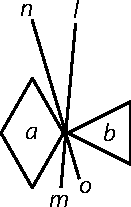
\includegraphics[width=0.14\textwidth]{gesamttex/edit_VIII-4/images/LH_37_05_043_d5_043v.pdf}}%
\vspace{1.0em}%
\centerline{\hspace{-90mm}%
\lbrack\textit{Fig.\:5}\rbrack}
\vspace{5.0em}%
\vspace{-15.65em} %
\centerline{\hspace{45mm}%
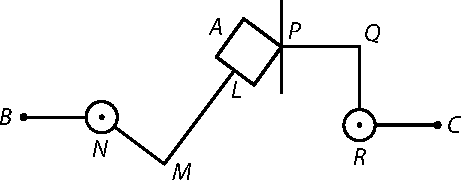
\includegraphics[width=0.5\textwidth]{gesamttex/edit_VIII-4/images/LH_37_05_043_d6_043v.pdf}}
\vspace{1.5em}
\centerline{\hspace{45mm}%
\lbrack\textit{Fig.\:6}\rbrack}
\vspace{3.5em}%
\pstart%
\noindent%
\lbrack\textit{Ohne unmittelbaren Zusammenhang mit dem Text und wohl bereits vorhanden:}\rbrack\
\pend%
\vspace*{2.5em} %
\centerline{\hspace{-05mm}%
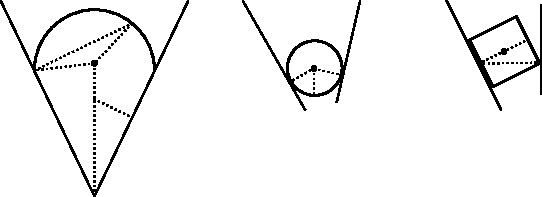
\includegraphics[width=0.52\textwidth]{gesamttex/edit_VIII-4/images/LH_37_05_043_d7_043v.pdf}}
\vspace{-1.0em}
\centerline{\hspace{-00mm}%
\lbrack\textit{Fig.\:7}\rbrack}
\vspace{2.5em} %
\centerline{\hspace{00mm}%
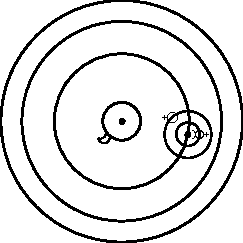
\includegraphics[width=0.26\textwidth]{gesamttex/edit_VIII-4/images/LH_37_05_043_d8_043v.pdf}}
\vspace{0.75em}
\centerline{\hspace{00mm}%
\lbrack\textit{Fig.\:8}\rbrack}
\selectlanguage{latin}%
\frenchspacing%
\normalsize%
